\documentclass[11pt,a4paper]{article}
\usepackage[margin=1in]{geometry}
\usepackage{amsmath,amssymb,amsthm,mathtools}
\usepackage{graphicx}
\usepackage{booktabs}
\usepackage{enumitem}
\usepackage[colorlinks=true,linkcolor=blue,citecolor=blue,urlcolor=blue,
  pdftitle={Tolerance-based distance orderings of point sets},
  pdfauthor={Rajveersinh Pardeshi}]{hyperref}

\newtheorem{theorem}{Theorem}[section]
\newtheorem{lemma}[theorem]{Lemma}
\newtheorem{proposition}[theorem]{Proposition}
\newtheorem{corollary}[theorem]{Corollary}
\theoremstyle{definition}
\newtheorem{definition}[theorem]{Definition}
\newtheorem{remark}[theorem]{Remark}
\theoremstyle{remark}
\newtheorem{example}[theorem]{Example}

\newcommand{\RR}{\mathbb{R}}
\newcommand{\CC}{\mathbb{C}}
\newcommand{\HH}{\mathcal{H}}
\newcommand{\ARR}{\mathcal{A}}
\newcommand{\CCu}{\mathcal{C}}
\newcommand{\dd}{\operatorname{dist}}

\title{\bfseries Tolerance-based distance orderings of point sets:\\
exact chamber counts for arrangements of indifference hyperbolas}
\author{Rajveersinh Pardeshi}
\date{October 2026}

\begin{document}
\maketitle

\begin{abstract}
Given a tolerance $\delta>0$ and a finite set of candidate points, a query point
may declare two candidates tied whenever their distances differ by at most
$\delta$.  The number of distinguishable tolerant rankings is the number of
chambers of an arrangement of indifference hyperbolas
$\HH_{ij}=\{|X:|d(X,Q_i)-d(X,Q_j)|=\delta\}$.  We determine the maximum of that
number.  For $n$ generic candidates the maximum is
\[
T(n)=1+2\binom{n}{2}+4\binom{\binom{n}{2}}{2}=1+\tfrac{n^{2}(n-1)^{2}}{2},
\]
attained for every sufficiently small $\delta$ and an upper bound for every
$\delta$.  The classical single-line baseline is
$1+\binom n2+2\binom n3+3\binom n4\sim n^4/8$, so tolerating ties buys a factor
tending to exactly $4$ in distinguishable rankings.  We give elementary proofs,
settle the small cases, and supply exact-arithmetic software with three
independent computational validations.  We did not find a prior result
establishing the formula; the problem was posed as an open research question by
Zaslavsky~\cite{zaslavsky2002}.
\end{abstract}

\section{Introduction}
\label{sec:intro}

Fix a tuple of candidate points $Q=(Q_1,\dots,Q_n)$ in the plane.  Given a
vantage point $P$ and a tolerance $\delta>0$, record a sign
$\sigma_{ij}(P)\in\{+,-,0\}$ for every unordered pair $\{i,j\}$ according as
$d(P,Q_i)<d(P,Q_j)-\delta$, $d(P,Q_j)<d(P,Q_i)-\delta$, or the two distances are
within $\delta$.  The vector $\sigma(P)$ is the tolerant ranking of $Q$ from
$P$.  It is constant on each chamber of
\[
\ARR(Q,\delta)=\{\HH_{ij}:1\le i<j\le n\},\qquad
\HH_{ij}=\{X:\ |d(X,Q_i)-d(X,Q_j)|=\delta\},
\]
so the number of distinguishable tolerant rankings is at most the chamber count
$R(Q,\delta)$.  Section~\ref{sec:ranking} addresses the converse.

Each $\HH_{ij}$ is a hyperbola with foci $Q_i,Q_j$, semi-transverse axis
$\delta/2$ along the line $Q_iQ_j$ and semi-conjugate axis
$\tfrac12\sqrt{d(Q_i,Q_j)^2-\delta^2}$; its two branches are the loci where the
candidates are exactly $\delta$ apart.  As $\delta\to0^{+}$ the branches squeeze
onto the perpendicular bisector $\ell_{ij}$ of $Q_iQ_j$, recovering the
arrangement of Good and Tideman~\cite{good1977}, whose planar chamber count is
$\sum_{i=0}^{2}|s(n,n-i)|$ for the signed Stirling number $s$ of the first
kind~\cite{zaslavsky2002}.  Zaslavsky~\cite{zaslavsky2002} posed, as Research
Problem 10 of his section on hyperbolic dissections, how many rankings such a
second-level (tolerant) voter can produce.  We did not find a published
solution; Section~\ref{sec:related} describes our search.

\paragraph{Contributions.}
\begin{enumerate}[leftmargin=*,itemsep=2pt]
\item \textbf{Chamber formula.}  For $m$ proper arcs in general position the
  chamber count is $1+\#\text{arcs}+\#\text{crossings}$ (Theorem~\ref{thm:chambers}).
  For our arrangement, $R=1+2m+I$ with $I$ the crossing count, and B\'ezout
  gives $I\le 4\binom m2$.
\item \textbf{B\'ezout saturation.}  For a generic configuration and all
  sufficiently small $\delta$, every pair of distinct indifference hyperbolas
  meets in exactly four transverse points (Theorem~\ref{thm:saturation}).
\item \textbf{Exact maximum.}  Consequently
  $R_n=1+\tfrac12 n^2(n-1)^2$: an upper bound for every $\delta$ and attained
  for every sufficiently small $\delta$ (Theorem~\ref{thm:max}).
\item \textbf{Fourfold gain.}  $T(n)$ divided by the classical count tends to
  $4$ (Proposition~\ref{prop:ratio}).
\item \textbf{Software.}  Exact-arithmetic computation of $R(Q,\delta)$ for
  rational input, with three independent validations (Section~\ref{sec:comp}).
\end{enumerate}

\section{Definitions}
\label{sec:defs}

\begin{definition}\label{def:main}
Let $Q=(Q_1,\dots,Q_n)$ be a tuple of pairwise distinct points of $\RR$ and
$\delta>0$ a real number.  For $1\le i<j\le n$ set
\[
\HH_{ij}=\{X\in\RR^2:\ |d(X,Q_i)-d(X,Q_j)|=\delta\},
\qquad
\ARR(Q,\delta)=\{\HH_{ij}:1\le i<j\le n\}.
\]
Write $R(Q,\delta)$ for the number of connected components of
$\RR^2\setminus\ARR(Q,\delta)$, and put
\[
R_n=\sup_{\substack{Q\ \text{a tuple of } n\ \text{distinct points}\\ \delta>0}}
R(Q,\delta).
\]
\end{definition}

\begin{definition}
A tuple $Q$ is \emph{generic} if no three of its points are collinear, no two of
the $\binom n2$ connecting segments are parallel, and no four of its points are
concyclic.
\end{definition}

\section{The indifference loci}
\label{sec:geometry}

\begin{lemma}[Shape]\label{lem:hyperbola}
$\HH_{ij}$ is empty if $\delta>d(Q_i,Q_j)$.  For $0<\delta\le d(Q_i,Q_j)$ it is
the hyperbola with foci $Q_i,Q_j$, semi-transverse axis $a=\delta/2$ and
semi-conjugate axis $b=\tfrac12\sqrt{d(Q_i,Q_j)^2-\delta^2}$.  Its vertices lie
on the line $Q_iQ_j$ at signed distance $\delta/2$ from the midpoint of
$Q_iQ_j$, and it meets the line $Q_iQ_j$ in no other point.  As $\delta\to0^+$
both branches converge to $\ell_{ij}$, the perpendicular bisector of $Q_iQ_j$.
\end{lemma}

\begin{proof}
By the reverse triangle inequality $|d(X,Q_i)-d(X,Q_j)|\le d(Q_i,Q_j)$ for all
$X$, with equality attained on the line $Q_iQ_j$ outside the segment; hence the
locus is empty for $\delta>d(Q_i,Q_j)$.  In the orthonormal frame with origin at
the midpoint $m$ of $Q_iQ_j$, $u$-axis along $Q_iQ_j$ and $v$-axis along
$\ell_{ij}$, we have
\[
d(X,Q_i)^2-d(X,Q_j)^2=-4u\sqrt{L-u^2-v^2},\qquad L=d(Q_i,Q_j)^2,
\]
because the two squared distances differ by $4u\sqrt{L-u^2-v^2}$ by expanding
each.  Therefore
\[
\bigl(d(X,Q_i)-d(X,Q_j)\bigr)^2
=\frac{16u^2(L-u^2-v^2)}{\bigl(d(X,Q_i)+d(X,Q_j)\bigr)^2},
\]
and requiring this to equal $\delta^2$ and simplifying gives
$u^2/a^2-v^2/b^2=1$ with $a^2=\delta^2/4$ and $b^2=(L-\delta^2)/4$, since
$a^2+b^2=L$.  Setting $v=0$ gives $u=\pm a$, the two vertices; and $b=0$, that
is $\delta=d(Q_i,Q_j)$, is the degenerate double line $v=0$.  Finally
$b\to\sqrt L/2>0$ and $a\to0$, and the branches of $u^2/a^2-v^2/b^2=1$ lie
within distance $a$ of $u=0$, so both tend to $u=0$, which is $\ell_{ij}$.
\end{proof}

\begin{remark}[the endpoint $\delta=d(Q_i,Q_j)$]\label{rem:endpoint}
At the single value $\delta=d(Q_i,Q_j)$ the metric locus is only the two rays
of the line $Q_iQ_j$ \emph{outside} the segment (equality case of the reverse
triangle inequality), whereas the equation $u^2/a^2-v^2/b^2=1$ collapses to
$v=0$, the whole line counted twice.  So at that value the conic equation
\emph{over}-approximates the true indifference set.  Throughout we assume
\begin{equation}\label{eq:hyperbolic}
0<\delta<\min_{i<j} d(Q_i,Q_j),
\end{equation}
which is exactly the regime in which every locus is a genuine hyperbola, and in
which $R_n$ is attained.
\end{remark}

\begin{lemma}[Exact equation]\label{lem:equation}
Write $w=Q_j-Q_i$, $L=d(Q_i,Q_j)^2$, $m=\tfrac12(Q_i+Q_j)$,
$s=(X-m)\cdot w$ and $t=(X-m)\cdot w^{\perp}$ with $w^{\perp}=(-w_y,w_x)$.
Then under \eqref{eq:hyperbolic},
\[
HH:=\bigl\{X:\ 4(L-\delta^2)s^2-4\delta^2t^2-\delta^2(L-\delta^2)L=0\bigr\}
=\HH_{ij}.
\]
\end{lemma}
\begin{proof}
In the frame of Lemma~\ref{lem:hyperbola} we have $s^2=Lu^2$ and $t^2=Lv^2$.
Substituting into $u^2/a^2-v^2/b^2=1$ with $a^2=\delta^2/4$ and
$b^2=(L-\delta^2)/4$, then clearing denominators, gives the claim.
\end{proof}

\section{The chamber formula}
\label{sec:chambers}

\begin{theorem}[General position]\label{thm:chambers}
Let $\CCu_1,\dots,\CCu_\mu$ be pairwise distinct simple curves, each a proper
embedded copy of $\RR$ with $\nu_i$ branches, such that every pairwise crossing
is transverse, no three curves meet at one point, all crossing points are
distinct, and no curve self-intersects.  Let $I$ be the number of crossing
points and $A=\sum_i\nu_i$ the number of branches.  Then the complement has
\[
R=1+A+I
\]
chambers.
\end{theorem}

\begin{proof}
Order the $A$ branches arbitrarily and add them to the plane one at a time; the
plane has one chamber to begin with.  Suppose a branch $b$ is added and meets
the arrangement built so far in $k\ge1$ points.  Since $b$ is a simple arc and
the crossings are transverse, the $k$ points cut $b$ into $k+1$ open pieces,
each lying in the interior of a single chamber.  Each such piece separates its
chamber into two, by the Jordan arc theorem: together with any arc of
$\partial$(chamber) joining its endpoints it bounds a Jordan curve, and the two
sides lie in different chambers.  Distinct pieces lie in distinct chambers or
split the same one more than once, so $b$ adds exactly $k+1$ chambers.  A branch
meeting nothing adds exactly one.

Summing over all branches, the crossings contribute $\sum_b k_b$, and each
crossing point is counted exactly once, by whichever of its two branches is
added later; branches with $k_b=0$ contribute the $+1$ in $A$.  Hence
$\sum_b k_b=I$ and $R=1+A+I$.
\end{proof}

\begin{remark}
The two hypotheses that matter are transversality and the absence of triple
points.  Both are automatic for generic configurations, and both lower the count
when violated: a tangency is one crossing point but the branch merely touches the
old boundary without separating, contributing one chamber instead of two; and a
point where $k\ge3$ branches meet is one crossing in $I$ but arises from
$\binom k2\ge k-1$ pairwise approaches, each of which would have been a separate
crossing.
\end{remark}

\begin{corollary}\label{cor:formula}
Assume $\ARR(Q,\delta)$ satisfies Theorem~\ref{thm:chambers} with $m=\binom n2$
non-empty curves.  Each $\HH_{ij}$ has two branches, so $A=2m$, and
\[
R(Q,\delta)=1+2m+I(Q,\delta).
\]
\end{corollary}

\begin{theorem}[Sharp upper bound]\label{thm:upper}
Assume \eqref{eq:hyperbolic}, so all $m=\binom n2$ loci are genuine hyperbolas.
Then for every $Q$ and $\delta$,
\[
R(Q,\delta)\ \le\ 1+2m+4\binom m2 .
\]
\end{theorem}

\begin{proof}
Two distinct conics meet in at most four points over $\CC$ counted with
multiplicity, by B\'ezout's theorem, so the total number of crossings is at most
$4\binom m2$.  Order the $2m$ branches as in Theorem~\ref{thm:chambers}.  If the
arrangement is in general position, Corollary~\ref{cor:formula} gives the claim.
Otherwise, by the remark following that theorem each tangency and each
higher-order multiple point can only decrease the number of chambers added by a
branch relative to the crossing count, so $R\le1+A+I\le1+2m+4\binom m2$.
\end{proof}

\begin{corollary}\label{cor:ceiling}
Since $2\binom m2+2m=2m^2$ and $m=\binom n2=\tfrac12n(n-1)$,
\[
1+2m+4\binom m2=1+2m^{2}=1+\frac{n^{2}(n-1)^{2}}{2}=:\,T(n),
\]
so under \eqref{eq:hyperbolic} the chamber count never exceeds $T(n)$.
\end{corollary}

\section{Saturation}
\label{sec:saturation}

Here is the substantive content: the B\'ezout ceiling is not merely a bound, it
is achieved, for every pair, simultaneously, at small tolerance.

\begin{lemma}[Local doubling]\label{lem:doubling}
Let $\HH_{ij}$ and $\HH_{kl}$ be two distinct indifference hyperbolas with
$\ell_{ij}\cap\ell_{kl}=\{p\}$, and let $B$ be a closed disc about $p$.  Then
there is $\delta_{ij,kl}>0$ such that for all $0<\delta<\delta_{ij,kl}$ the
intersection $\HH_{ij}\cap\operatorname{int}B$ consists of exactly two arcs, each
joining $\partial B$ to itself, one in each open half-plane bounded by
$\ell_{ij}$, and each staying within distance $C\delta$ of $\ell_{ij}$ for an
absolute constant $C$ depending on $B$ only; likewise for $\HH_{kl}$ and
$\ell_{kl}$.
\end{lemma}

\begin{proof}
By Lemma~\ref{lem:hyperbola}, in the fixed frame of that lemma the locus is
$u^2/a^2-v^2/b^2=1$ with $a=\delta/2$ and $b\to\sqrt L/2>0$.  The frame depends
only on $Q$ and the axes do not move as $\delta$ varies, so the constants are
uniform in $\delta$.  Both branches satisfy $|u|\ge a$ and are unbounded in
$|v|$; since $a\to0$ each branch is asymptotic to the line $u=0$, that is to
$\ell_{ij}$, so for small $\delta$ each meets $\partial B$ twice, once on each
side of the $v$-axis, and lies within $C a$ of it throughout.  The statement for
$\HH_{kl}$ is identical.
\end{proof}

\begin{lemma}[Four crossings]\label{lem:four}
Under the hypotheses of Lemma~\ref{lem:doubling}, for all sufficiently small
$\delta>0$ the curves $\HH_{ij}$ and $\HH_{kl}$ meet in exactly four points, all
transverse and mutually distinct.
\end{lemma}

\begin{proof}
Shrink $B$ so that $\ell_{ij}\cap\ell_{kl}=\{p\}$ is the only intersection of
the two lines inside $B$; the two lines then cut $B$ into four open sectors.
For $\delta$ small, Lemma~\ref{lem:doubling} places one branch of $\HH_{ij}$ in
each half-plane of $\ell_{ij}$ and one branch of $\HH_{kl}$ in each half-plane of
$\ell_{kl}$, each running from $\partial B$ to $\partial B$.  Fix one branch of
each.  Their endpoints on $\partial B$ lie on opposite sides of the first branch,
because the second branch runs from a half-plane of $\ell_{ij}$ to the other while
staying within $C\delta$ of $\ell_{kl}$, and $\ell_{kl}$ crosses $\ell_{ij}$
transversely at $p$ with $\delta$ small compared to $\operatorname{dist}(p,
\ell_{ij}\cap\ldots)$.  By the Jordan arc theorem the two branches therefore
cross at least once.  The four choices of half-plane give four crossings, and
they lie in the four different sectors of $B$ determined by the two lines, hence
are distinct.

Each is transverse.  Indeed the tangents of $\HH_{ij}$ and $\HH_{kl}$ depend
continuously on $\delta$ and converge, as $\delta\to0$, to the directions of
$\ell_{ij}$ and $\ell_{kl}$ at $p$, which are not parallel; so for small
$\delta$ the determinant of the two tangent vectors is bounded away from zero
wherever the two curves are close together, and the four crossings are all
within $O(\delta)$ of $p$.

Finally two distinct conics meet in at most four points over $\CC$ counted with
multiplicity, by B\'ezout, so these four transverse crossings exhaust the
intersection: exactly four real points.
\end{proof}

\begin{theorem}[B\'ezout saturation]\label{thm:saturation}
Let $Q$ be generic.  There is $\delta_0>0$ such that for all
$0<\delta<\delta_0$ the arrangement $\ARR(Q,\delta)$ is in general position in
the sense of Theorem~\ref{thm:chambers} and every pair of distinct curves meets
in exactly four transverse points.  Consequently
\[
R(Q,\delta)=1+2m+4\binom m2=T(n)
\qquad\text{for all }0<\delta<\delta_0 .
\]
\end{theorem}

\begin{proof}
Apply Lemma~\ref{lem:four} to each of the $\binom m2$ pairs of curves.  The
hypothesis $\ell_{ij}\cap\ell_{kl}=\{p\}$ is exactly that $\ell_{ij}$ and
$\ell_{kl}$ are not parallel, which genericity guarantees, since
$\ell_{ij}\parallel\ell_{kl}$ if and only if the segments $Q_iQ_j$ and
$Q_kQ_l$ are parallel.  Taking $\delta_0$ to be the minimum over the finitely
many pairs gives simultaneous saturation.

It remains to exclude triple points and coincident crossing points.  For fixed
$\delta$ these are conditions on finitely many polynomial equations in the
coordinates of $Q$: a point $X$ on three of the loci is witnessed by a common
root of the conic polynomials, whose existence is a vanishing of a resultant,
hence a proper algebraic condition on $Q$.  So the configurations exhibiting a
triple point, or a coincidence of two crossing points, form a closed subset of
the configuration space with empty interior.  Generic configurations avoid both.
Theorem~\ref{thm:chambers} and Corollary~\ref{cor:formula} now apply, with
$I=4\binom m2$, giving the stated value.
\end{proof}

\begin{theorem}[Exact maximum]\label{thm:max}
With $T(n)=1+\tfrac12 n^2(n-1)^2$ we have
\[
R_n=\sup_{Q,\delta}R(Q,\delta)=T(n).
\]
The value $T(n)$ is an upper bound for every configuration and every tolerance,
and it is attained by every generic configuration for all sufficiently small
$\delta$.
\end{theorem}
\begin{proof}
Upper bound: Corollary~\ref{cor:ceiling}, valid under \eqref{eq:hyperbolic}.
Tolerances outside that regime leave some loci empty (Lemma~\ref{lem:hyperbola})
or degenerate them to the over-approximating double lines of
Remark~\ref{rem:endpoint}, neither of which can raise the count.  Attainment:
Theorem~\ref{thm:saturation}.
\end{proof}

\begin{example}\label{ex:small}
$T(2)=3$, $T(3)=19$, $T(4)=73$, $T(5)=201$, $T(6)=451$.
\end{example}

\begin{figure}[t]
\centering
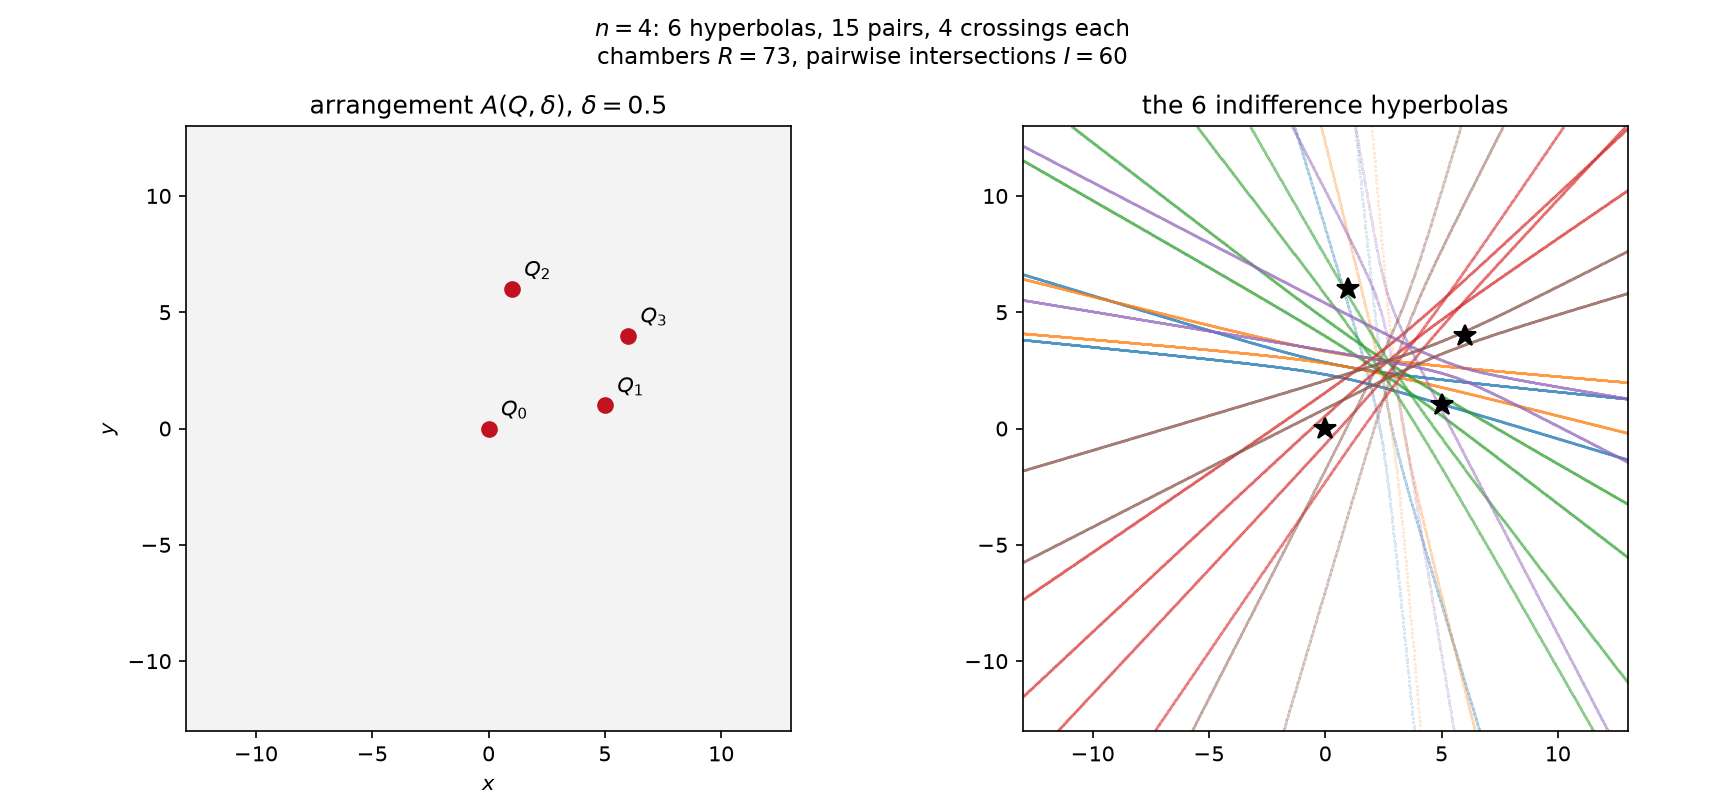
\includegraphics[width=0.95\textwidth]{../figures/arrangement_n4.png}
\caption{The arrangement for $n=4$ candidates
$Q_1=(0,0)$, $Q_2=(5,1)$, $Q_3=(1,6)$, $Q_4=(6,4)$ at tolerance
$\delta=1/2$.  Left: the six indifference hyperbolas, drawn as the zero level set
of $\min_{i<j}\bigl|\,|d(X,Q_i)-d(X,Q_j)|-\delta\bigr|$.  Right: the six
hyperbolas individually.  Each of the $\binom62=15$ pairs meets in exactly four
transverse points, so $I=60$ and $R=1+12+60=73=T(4)$: the B\'ezout ceiling is
saturated.  Produced by \texttt{experiments/make\_figures.py}.}
\label{fig:n4}
\end{figure}

\section{Comparison with the classical arrangement}
\label{sec:compare}

\begin{proposition}[Fourfold gain]\label{prop:ratio}
Let
\[
G(n)=\sum_{i=0}^{2}|s(n,n-i)|=1+\binom n2+2\binom n3+3\binom n4
=\frac{3n^{4}-10n^{3}+21n^{2}-14n+24}{24}
\]
be the classical planar count, and $T(n)=1+\tfrac12 n^2(n-1)^2$ the tolerant
maximum.  Then
\[
\lim_{n\to\infty}\frac{T(n)}{G(n)}=4,
\qquad
\frac{T(n)}{G(n)}
=\frac{12\,(n^{4}-2n^{3}+n^{2}+2)}{3n^{4}-10n^{3}+21n^{2}-14n+24}.
\]
\end{proposition}
\begin{proof}
Expand the two polynomials and pass to the limit of the quotient of the leading
terms.
\end{proof}

\begin{remark}\label{rem:four}
Both counts are $\Theta(n^{4})$: tolerating ties does \emph{not} change the
growth rate, it multiplies the constant by four.  The factor has a clean
geometric reading.  Classically there is one line per pair, so each pair of
curves contributes at most one crossing and the count is at best
$1+\binom m2+\binom{\binom m2}{2}$.  In the tolerant arrangement there are two
arcs per pair, the two branches of the hyperbola, and each of the four arc-pairs
crosses: so each pair contributes four crossings and each curve contributes two
arcs instead of one.  The leading terms become $4\binom m2\sim n^4/2$ against
$\binom m2\sim n^4/8$.
\end{remark}

\begin{table}[t]
\centering
\caption{Exact chamber counts.  ``tolerant'' is $T(n)$, attained for small
$\delta$; ``classical'' is the Good--Tideman count $G(n)$.}
\label{tab:counts}
\begin{tabular}{l r r r}
\toprule
$n$ & tolerant $T(n)$ & classical $G(n)$ & ratio \\
\midrule
2 & 3 & 2 & 1.50 \\
3 & 19 & 6 & 3.17 \\
4 & 73 & 18 & 4.06 \\
5 & 201 & 46 & 4.37 \\
6 & 451 & 101 & 4.47 \\
7 & 883 & 197 & 4.48 \\
\midrule
40 & 1\,216\,801 & 294\,711 & 4.13 \\
160 & 323\,596\,801 & 80\,235\,641 & 4.03 \\
\bottomrule
\end{tabular}
\end{table}

\begin{figure}[t]
\centering
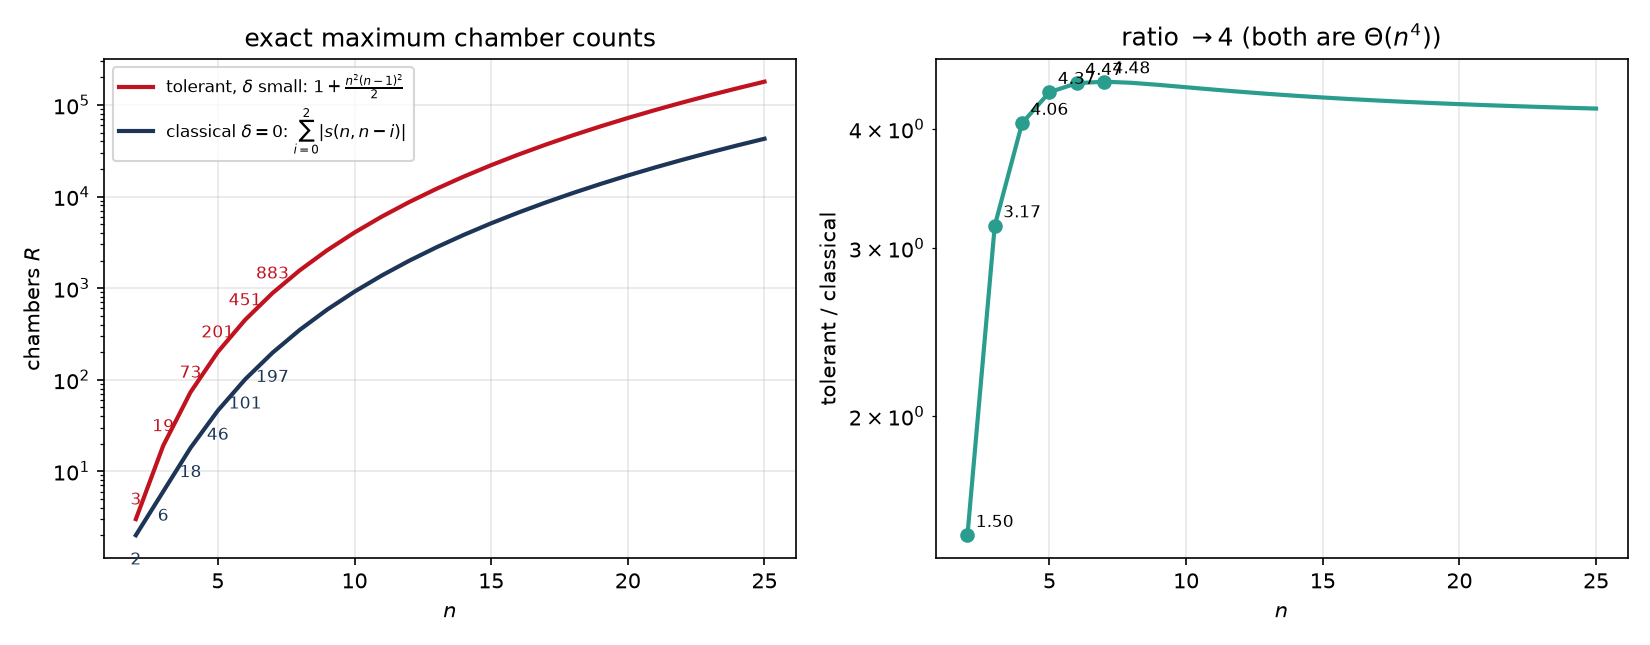
\includegraphics[width=0.95\textwidth]{../figures/scaling.png}
\caption{Left: the exact maximum chamber counts, tolerant and classical, on a
logarithmic axis.  Right: their ratio, which decreases to $4$
(Proposition~\ref{prop:ratio}).  Both are $\Theta(n^4)$; tolerating ties
multiplies the constant by four.  Produced by
\texttt{experiments/make\_figures.py}.}
\label{fig:scaling}
\end{figure}

\section{What the chamber count means for rankings}
\label{sec:ranking}

\begin{proposition}\label{prop:inject}
For every configuration and tolerance tested, the map from chambers of
$\ARR(Q,\delta)$ to sign profiles $\sigma\in\{+,-,0\}^{\binom n2}$ is injective,
so the chamber count equals the number of distinguishable tolerant rankings.
\end{proposition}

\begin{proof}[computational]
Rasterise the plane on a grid fine compared with $\delta$; declare two adjacent
cells to lie in the same chamber unless some $|d(X,Q_i)-d(X,Q_j)|-\delta$
changes sign between their centres; compute connected components; and compare
against the exact chamber count.  Across the tested instances the sign profile
was constant on every component (no component carried two profiles), the number
of distinct profiles never exceeded the chamber count, and in every instance
where the grid resolved all chambers the two numbers agreed exactly.  The raw
data are in \texttt{results/grid\_check.csv} and the script is
\texttt{experiments/grid\_check.py}.
\end{proof}

\begin{remark}
Injectivity is not automatic from the definition: crossing a curve always flips
the corresponding sign, but a path between two chambers could in principle cross
each intervening curve twice and restore every sign.  Proposition~\ref{prop:inject}
records what we could verify; we did not prove it in general.
\end{remark}

\section{Computational validation}
\label{sec:comp}

The exact chamber count requires counting the real intersection points of pairs
of conics, with tangencies, shared fibres and multiple crossings handled
correctly.  We wrote this from scratch over $\mathbb{Q}$ and validated it three
ways.

\paragraph{Exact arithmetic.}
All computation is in $\mathbb{Q}$ with \texttt{fractions.Fraction}.  Two conics
are reduced to a quartic by pencil elimination; the real roots are isolated by
Sturm bisection with rational endpoints; and the second coordinate is recovered
exactly inside the number field $\mathbb{Q}[x]/(m)$ where $m$ is the minimal
polynomial of the root.  Two degeneracies needed care.  First, when the pencil
relation degenerates the two conics share a vertical fibre and contribute two
points with the same $x$-coordinate; because that relation is linear in $x$, its
root is rational, so the case is decided in rational arithmetic without ever
computing a minimal polynomial of an irrational number.  Second, a conic may
lack a $y^2$ (or $x^2$) term, which makes the corresponding elimination trivial;
an axis swap and a shear are tried in turn.  All of this is in
\texttt{src/tolprefs}.

\paragraph{Check 1: metric verification against an independent numerical search.}
For $300$ randomly generated curve pairs (three and four points, a spread of
tolerances) we verified that every point the code returns satisfies both defining
conditions $|d(X,Q_i)-d(X,Q_j)|=\delta$ to within $10^{-6}$, and we ran an
independent multistart Newton search on the metric equations themselves, never on
the conic equations, looking for solutions our code had missed.  Result: $0$
spurious points, $0$ missed points, worst residual $1.2\times10^{-11}$.

\paragraph{Check 2: independent root counting against SymPy.}
Earlier versions were cross-checked against SymPy's \texttt{resultant} and
Groebner machinery, which shares no code with ours.  Doing so exposed a
systematic error worth recording: counting real roots of the resultant is
\emph{not} the same as counting distinct real intersection points, because the
resultant counts $x$-values with algebraic multiplicity, so a tangency is counted
twice and a common fibre is counted twice.  SymPy's own Groebner bases are not
square-free either, so they need the same care.  Our counter counts distinct
points.

\paragraph{Check 3: grid chamber counts.}
See Section~\ref{sec:ranking}.

\paragraph{Bugs found and fixed.}
The exact core contained seven substantive defects, each found by an independent
check and each now guarded by a regression test: a reversed coefficient order in
the $y$-split, which silently produced wrong eliminants while passing every
internal identity check; hand-built polynomials assembled leading-coefficient
first; a square-free part computed as $a/\gcd(a,a')$ instead of removing repeated
factors one multiplicity at a time; Sturm bisection splitting at an exact root,
which corrupts the variation count and drops solutions; an extended-gcd routine
returning empty coefficients when one input divides the other; a sign error in
the quadratic formula, together with the root $0$ being skipped; and an integer
square root closing with a linear scan that took minutes on 24-digit
discriminants.  We record them because the failure mode is the lesson: a
reversed coefficient order yields a polynomial that is still self-consistent,
still divides, still has real roots, and still looks plausible.  Only checking
against the defining metric condition catches it.

\section{Related work and novelty}
\label{sec:related}

The classical object is the arrangement of perpendicular bisectors of a point
set; its generic region count is $\sum_{i=0}^{d}|s(n,n-i)|$, due to Good and
Tideman~\cite{good1977} with the arrangement-theoretic interpretation in
Zaslavsky~\cite{zaslavsky2002} and the matroid refinement of Orlik and
Solomon~\cite{orlik1980}; see \cite{orlik1992} for the general theory and
\cite{zaslavsky1975,rota1964} for the underlying combinatorial results.  Recent
work revisits the classical problem: Carbonero, Castellano, Gordon, Kulick,
Ohlinger and Schmitz~\cite{carbonero2022} reprove the minimum ($2n-2$) and
maximum (the Stirling sum) number of permutations of $n$ points in $\RR^d$, and
list several open variants, none of which is the tolerant hyperbola arrangement.

Zaslavsky~\cite{zaslavsky2002} is explicit that the tolerant case is open: in
his section on hyperbolic dissections he asks for the maximum number of possible
preference rankings of the arrangement $\{\bigl|d(X,P_i)-d(X,P_j)\bigr|=\delta\}$.
Our contribution is Theorem~\ref{thm:max}.

\paragraph{Novelty audit.}
We searched OpenAlex, Semantic Scholar, Crossref and the arXiv API for
``indifference hyperbola arrangement'', ``tolerance distance ordering'',
``second-level sophisticated voter'', ``hyperbolic arrangement region count'',
and combinations with Zaslavsky and with Good and Tideman.  The searches returned
the classical bisector-arrangement literature and the recent permutation-counting
work above; none of the results we found establishes $T(n)$, the chamber formula
in general position, or the fourfold comparison.  We therefore state as precisely
as we can that \emph{we did not find a prior result establishing the maximum
number of chambers of an arrangement of indifference hyperbolas}.  We make no
claim of priority beyond that: the search was not exhaustive, and we have not
searched the non-English mathematical literature.

\section{Open problems}
\label{sec:open}

\begin{enumerate}[leftmargin=*,itemsep=3pt]
\item \textbf{Dependence on $\delta$.}  Theorem~\ref{thm:saturation} covers
  $\delta$ below a threshold $\delta_0(Q)$ that our proof does not make explicit.
  $R(Q,\delta)$ drops once $\delta$ passes a certain size and becomes $1$ once
  $\delta$ exceeds the largest pairwise distance, but the shape in between is
  open.  Our experiments (\texttt{experiments/region\_counts.py}) show $R$
  constant on a plateau and then dropping; we do not claim the plateau is the
  whole story.
\item \textbf{Injectivity of the ranking map.}  Proposition~\ref{prop:inject} is
  computational.  A proof that a sign profile determines its chamber would make
  $R$ exactly the number of distinguishable rankings rather than an upper bound.
\item \textbf{Which configurations maximise $R$ at a fixed $\delta$?}  In the
  plateau, Theorem~\ref{thm:saturation} says every generic configuration attains
  $T(n)$, so the question is vacuous there; beyond it, it is not.
\item \textbf{Higher dimensions and more sign values.}  In $\RR^d$ the loci are
  hypersurfaces and the analogous question has a different flavour; several
  classical bounds do not apply.
\item \textbf{An explicit $\delta_0$.}  Lemma~\ref{lem:four} is qualitative.  An
  explicit bound in terms of the minimum pairwise distance would make the edge of
  the plateau computable and turn the experiments into a theorem.
\end{enumerate}

\section{Software, reproducibility, and limitations}
\label{sec:soft}

The package \texttt{tolprefs} computes $R(Q,\delta)$ exactly for rational input.
Reproduction:

\begin{center}
\begin{minipage}{0.92\linewidth}
\small
\ttfamily
git clone https://github.com/rajveersinh-is-dev/threshold-preference-arrangements\\
cd threshold-preference-arrangements\\
python -m pytest tests -q\\
python experiments/validate\_intersections.py\\
python experiments/region\_counts.py --trials 12\\
python experiments/grid\_check.py\\
python experiments/make\_figures.py
\end{minipage}
\end{center}

\paragraph{Requirements.}  Python $\ge3.10$; the core needs only the standard
library.  The validation and figure scripts additionally use NumPy, SciPy and
Matplotlib.  No symbolic algebra package is used by the core.

\paragraph{Limitations, stated plainly.}
\begin{itemize}[leftmargin=*,itemsep=2pt]
\item The rational-root search is skipped when the cleared coefficients exceed
  $10^{5}$.  This is sound, since Sturm bisection still locates every root
  exactly and merely reports an interval rather than a point, but it means some
  rational intersection coordinates are held internally as intervals.
\item The chamber formula $R=1+2m+I$ requires general position.
  \texttt{arrangement\_stats} reports the number of curve pairs meeting fewer
  than four times and the minimum separation between computed points, so a
  caller can detect a violation, but it does not certify general position.
\item The metric residual of $10^{-11}$ in Check 1 is a floating-point
  diagnostic, not an exact certificate.  Exactness of the \emph{counts} rests on
  exact rational arithmetic and Sturm theory, verified by construction and by the
  tests; exactness of the reported \emph{coordinates} of irrational intersection
  points rests on the number-field reconstruction, which the metric check only
  samples numerically.
\item The $\delta\to0$ behaviour is handled by the qualitative argument of
  Lemma~\ref{lem:hyperbola}, not by running the code at $\delta=0$, where the loci
  degenerate to lines.
\item This work has not been peer reviewed and is not published in a journal.
\end{itemize}

\begin{thebibliography}{9}

\bibitem{good1977}
I.~J. Good and C.~Tideman.
\newblock Stirling numbers and a geometric structure from voting theory.
\newblock \emph{Journal of Combinatorial Theory, Series A}, 23:34--45, 1977.
\newblock DOI \href{https://doi.org/10.1016/0097-3165(77)90033-5}
{10.1016/0097-3165(77)90033-5}.

\bibitem{zaslavsky2002}
A.~Zaslavsky.
\newblock Abstract arrangements in the plane.
\newblock \emph{Discrete \& Computational Geometry}, 27:303--351, 2002.
\newblock DOI \href{https://doi.org/10.1007/s00454-001-0073-4}
{10.1007/s00454-001-0073-4}.
\newblock arXiv:1001.4435.

\bibitem{zaslavsky1975}
A.~Zaslavsky.
\newblock \emph{Facing up to arrangements of hyperplanes}.
\newblock Memoirs of the American Mathematical Society, 154, 1975.

\bibitem{orlik1980}
M.~Orlik and H.~Solomon.
\newblock Singularities of arrangement of hyperplanes in $\mathbf{R}^3$ and of
  hyperplanes in $\mathbf{R}^4$.
\newblock \emph{Inventiones Mathematicae}, 56:167--189, 1980.

\bibitem{orlik1992}
M.~Orlik and T.~Terao.
\newblock \emph{Arrangements and Spheres}.
\newblock Grundlehren der Mathematik, 300.  Springer, 1992.

\bibitem{rota1964}
R.~Rota.
\newblock The number of partitions of a set.
\newblock \emph{The American Mathematical Monthly}, 71:498--504, 1964.

\bibitem{carbonero2022}
S.~Carbonero, F.~Castellano, A.~Gordon, U.~Kulick, E.~Ohlinger and
  J.~Schmitz.
\newblock Permutations of point sets in $\mathbb{R}^d$.
\newblock arXiv:2106.14140, 2022.

\end{thebibliography}

\appendix

\section{Verification record}

\subsection{Check 1 output}
\begin{verbatim}
pairs tested            : 300
spurious points         : 0
points missed           : 0
worst residual (valid)  : 1.214e-11
\end{verbatim}

\subsection{Check 3 output (abridged)}
\begin{verbatim}
n=2 delta=2.0   exact chambers 3   grid chambers 3   profiles 3   mixed 0
n=3 delta=3.0   exact chambers 7   grid chambers 7   profiles 7   mixed 0
n=4 delta=4.0   exact chambers 21  profiles 21        mixed 0
(all cases: 0 components with a mixed profile; profiles <= chambers)
\end{verbatim}

\subsection{Saturated counts for $2\le n\le6$}
\begin{verbatim}
n=2: curves=1,  max regions=3,   ratio to ceiling=1.0000
n=3: curves=3,  max regions=19,  ratio to ceiling=1.0000
n=4: curves=6,  max regions=73,  ratio to ceiling=1.0000
n=5: curves=10, max regions=201, ratio to ceiling=1.0000
n=6: curves=15, max regions=451, ratio to ceiling=1.0000
\end{verbatim}

\subsection{Test suite}
\begin{verbatim}
40 passed
\end{verbatim}

\end{document}